\documentclass[tikz,border=4pt]{standalone}
% Shared style for every figure and for the deck: one accent, one
% highlight, thin lines, rounded nodes, nothing decorative.
\usepackage[T1]{fontenc}
\usepackage{lmodern}
\renewcommand{\familydefault}{\sfdefault}
\usepackage{tikz}
\usetikzlibrary{arrows.meta,positioning,calc,shapes.misc,fit,backgrounds,decorations.pathreplacing}
\definecolor{ink}{RGB}{40,40,40}
\definecolor{soft}{RGB}{150,150,150}
\definecolor{faint}{RGB}{225,225,225}
\definecolor{accent}{RGB}{0,95,115}
\definecolor{accentlight}{RGB}{214,232,236}
\definecolor{warn}{RGB}{196,84,40}
\definecolor{warnlight}{RGB}{247,226,216}
\tikzset{
  every picture/.style={color=ink, line width=0.5pt, font=\small},
  node distance=12mm and 18mm,
  box/.style={draw=ink, rounded corners=2pt, fill=white, inner sep=5pt, minimum height=7mm, align=center},
  maker/.style={box, minimum width=18mm},
  cat/.style={box, inner sep=3.5pt, minimum height=6mm},
  root/.style={box, fill=accentlight, draw=accent},
  bad/.style={box, fill=warnlight, draw=warn},
  ghost/.style={box, draw=soft, text=soft, dashed},
  flow/.style={-{Stealth[length=4pt,width=3.5pt]}, line width=0.5pt},
  sub/.style={-{Stealth[length=4pt,width=3.5pt]}, line width=0.5pt, color=soft},
  strong/.style={flow, color=accent, line width=0.8pt},
  wrong/.style={flow, color=warn},
  lbl/.style={font=\footnotesize, text=ink, inner sep=1.5pt, fill=white},
  note/.style={font=\footnotesize, text=soft, align=center},
  rate/.style={font=\footnotesize, text=accent, inner sep=1pt, fill=white},
}

\usepackage{amsmath}
\usepackage{pgfplots}
\pgfplotsset{compat=1.17}

\begin{document}
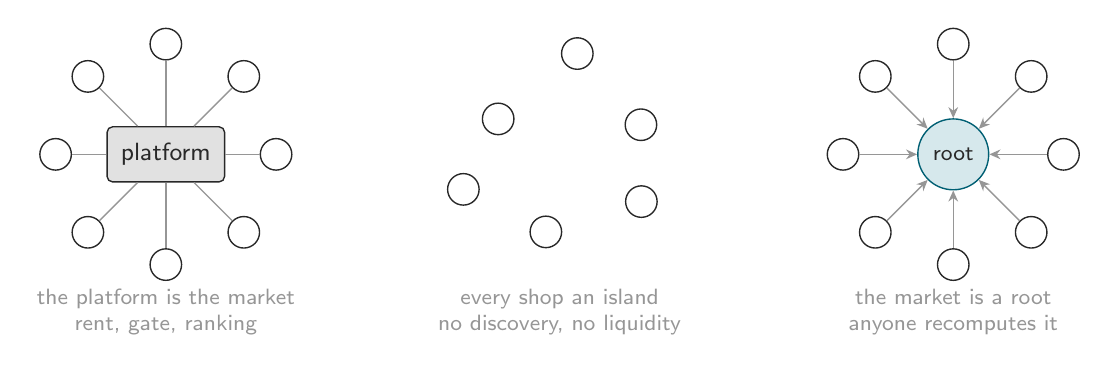
\begin{tikzpicture}[shop/.style={circle, draw=ink, fill=white, minimum size=4mm, inner sep=0pt}]
  % platform
  \begin{scope}
    \node[box, fill=faint] (P) {platform};
    \foreach \a in {0,45,...,315} { \node[shop] (s\a) at (\a:14mm) {}; \draw[soft] (P) -- (s\a); }
    \node[note] at (0,-20mm) {the platform is the market\\ rent, gate, ranking};
  \end{scope}
  % islands
  \begin{scope}[xshift=50mm]
    \foreach \a/\r in {20/11,80/13,150/9,200/13,260/10,330/12} { \node[shop] at (\a:\r mm) {}; }
    \node[note] at (0,-20mm) {every shop an island\\ no discovery, no liquidity};
  \end{scope}
  % shared root
  \begin{scope}[xshift=100mm]
    \node[root, circle, minimum size=9mm, inner sep=0pt, font=\footnotesize] (R) {root};
    \foreach \a in {0,45,...,315} { \node[shop] (t\a) at (\a:14mm) {}; \draw[sub] (t\a) -- (R); }
    \node[note] at (0,-20mm) {the market is a root\\ anyone recomputes it};
  \end{scope}
\end{tikzpicture}
\end{document}
